\documentclass[default]{beamer}
\setbeamertemplate{navigation symbols}{}

\usetheme{CambridgeUS}
\useoutertheme{infolines}
%\usecolortheme{crane}

\usepackage{cmap}							% Поддержка поиска русских слов в PDF (pdflatex)
\usepackage[T2A]{fontenc}       			%поддержка кириллицы
\usepackage[utf8]{inputenc}					% Выбор языка и кодировки
\usepackage[english, russian]{babel}
\usepackage{csquotes}
\usepackage{tikz}
\usetikzlibrary{arrows,shapes,calc}
\usepackage{animate}
\usepackage{fp}

\usepackage[
	language=auto,
	autolang=other,
	backend=biber,
	style=authortitle,
	sorting=ydnt,
	maxbibnames=5
]{biblatex}
\addbibresource{panov-cogconf.bib}
				
\DeclareSourcemap{
	\maps[datatype=bibtex, overwrite]{
		\map{
			\step[fieldset=langid, fieldvalue=english]
			\step[fieldset=doi, null]
			\step[fieldset=issn, null]
			\step[fieldset=isbn, null]
			\step[fieldset=url, null]
			\step[fieldsource=language, fieldset=langid, origfieldval]
		}
	}
}
\DeclareBibliographyDriver{std}{%
	\usebibmacro{bibindex}%
	\usebibmacro{begentry}%
	\usebibmacro{author/editor+others/translator+others}%
	\setunit{\labelnamepunct}\newblock
	\usebibmacro{title}%
	\newunit\newblock
	\usebibmacro{maintitle+booktitle}
	\newunit\newblock
	\usebibmacro{journal}%
	\newunit\newblock
	\usebibmacro{date}%
	\newunit\newblock
	\usebibmacro{finentry}
}
\DeclareBibliographyAlias{article}{std}
\DeclareBibliographyAlias{book}{std}
\DeclareBibliographyAlias{inproceedings}{std}
\DeclareBibliographyAlias{incollection}{std}

\graphicspath{{../../images/}} 			% Пути к изображениям

\makeatletter
\setbeamertemplate{footline}
{
	\leavevmode%
	\hbox{%
		\begin{beamercolorbox}[wd=.333333\paperwidth,ht=2.25ex,dp=1ex,center]{author
				in head/foot}%
			\usebeamerfont{author in
				head/foot}\insertshortauthor~~\beamer@ifempty{\insertshortinstitute}{}{(\insertshortinstitute)}
		\end{beamercolorbox}%
		\begin{beamercolorbox}[wd=.333333\paperwidth,ht=2.25ex,dp=1ex,center]{title in
				head/foot}%
			\usebeamerfont{title in head/foot}\insertshorttitle
		\end{beamercolorbox}%
		\begin{beamercolorbox}[wd=.333333\paperwidth,ht=2.25ex,dp=1ex,right]{date in
				head/foot}%
			\usebeamerfont{date in head/foot}\insertshortdate{}\hspace*{2em}
			\insertframenumber{}\hspace*{2ex} 
		\end{beamercolorbox}
	}%
	\vskip0pt%
}

\newcommand{\predmatr}[3]{
	\node[ell, rectangle, minimum height = 15, minimum width = 7.5]  at (#1 pt,#2 pt) {}; 
	\node[ellf, rectangle, minimum height = 15, minimum width = 7.5] at (#1+7.5 pt,#2 pt) {};
	\node[minimum height = 15, minimum width = 15] (#3) at (#1+3.3pt,#2 pt) {};
	\draw[ell] (#1+7.5 pt,#2+7.5 pt) -- (#1 +7.5 pt,#2-7.5 pt);
}
\renewcommand*{\bibfont}{\tiny}
\setlength\bibitemsep{-5pt}

\begin{document}
	
	\title[Планирование в картине мира]{Моделирование процесса планирования поведения в знаковой картине мира}
	\author[Панов]{Александр Панов}
	\institute[ФИЦ ИУ РАН]{Федеральный исследовательский центр <<Информатика и управление>>\\Российской академии наук}
	\date{23 июня 2016~г.} 
	
	\begin{frame}
		\titlepage
	\end{frame}

	\section{Знаковая модель}
	\begin{frame}
		\frametitle{Знаковая модель представления знаний}
		{\footnotesize
			Компонентом представления знаний является знак:
			\begin{itemize}
				\item в смысле культурно-исторического подхода Выготского-Лурии,
				\item следуя теории деятельности Леонтьева.
			\end{itemize}
		}
		\begin{columns}
			\begin{column}{0.4\textwidth}
				\centering
				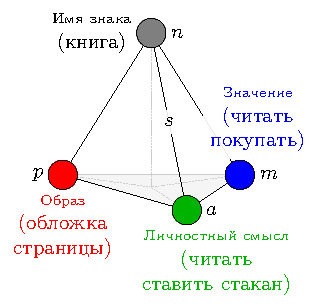
\includegraphics[width=0.7\textwidth]{signs/sign_color_book_ru}
			\end{column}
			\begin{column}{0.6\textwidth}
				\centering
				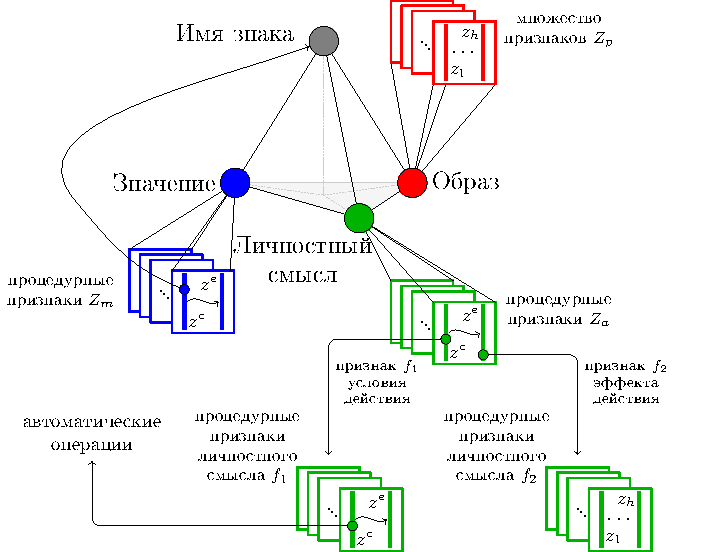
\includegraphics[width=0.6\textwidth]{signs/sign_details2_ru}
			\end{column}
		\end{columns}
		
		{\footnotesize
		В пользу существования такой структуры свидетельствуют:
		\begin{itemize}
			\item нейрофизиологические данные (Эдельман, Иваницкий, Маунткастл и др.),
			\item другие психологические теории (например, трехкомпонентная модель Станович).
		\end{itemize}
		}
		\vspace{-5pt}
		\nocite{*}
		\printbibliography[keyword={sign}, resetnumbers=true]
	\end{frame}

	\begin{frame}
		\frametitle{Уровни представления}
		
		\begin{figure}
			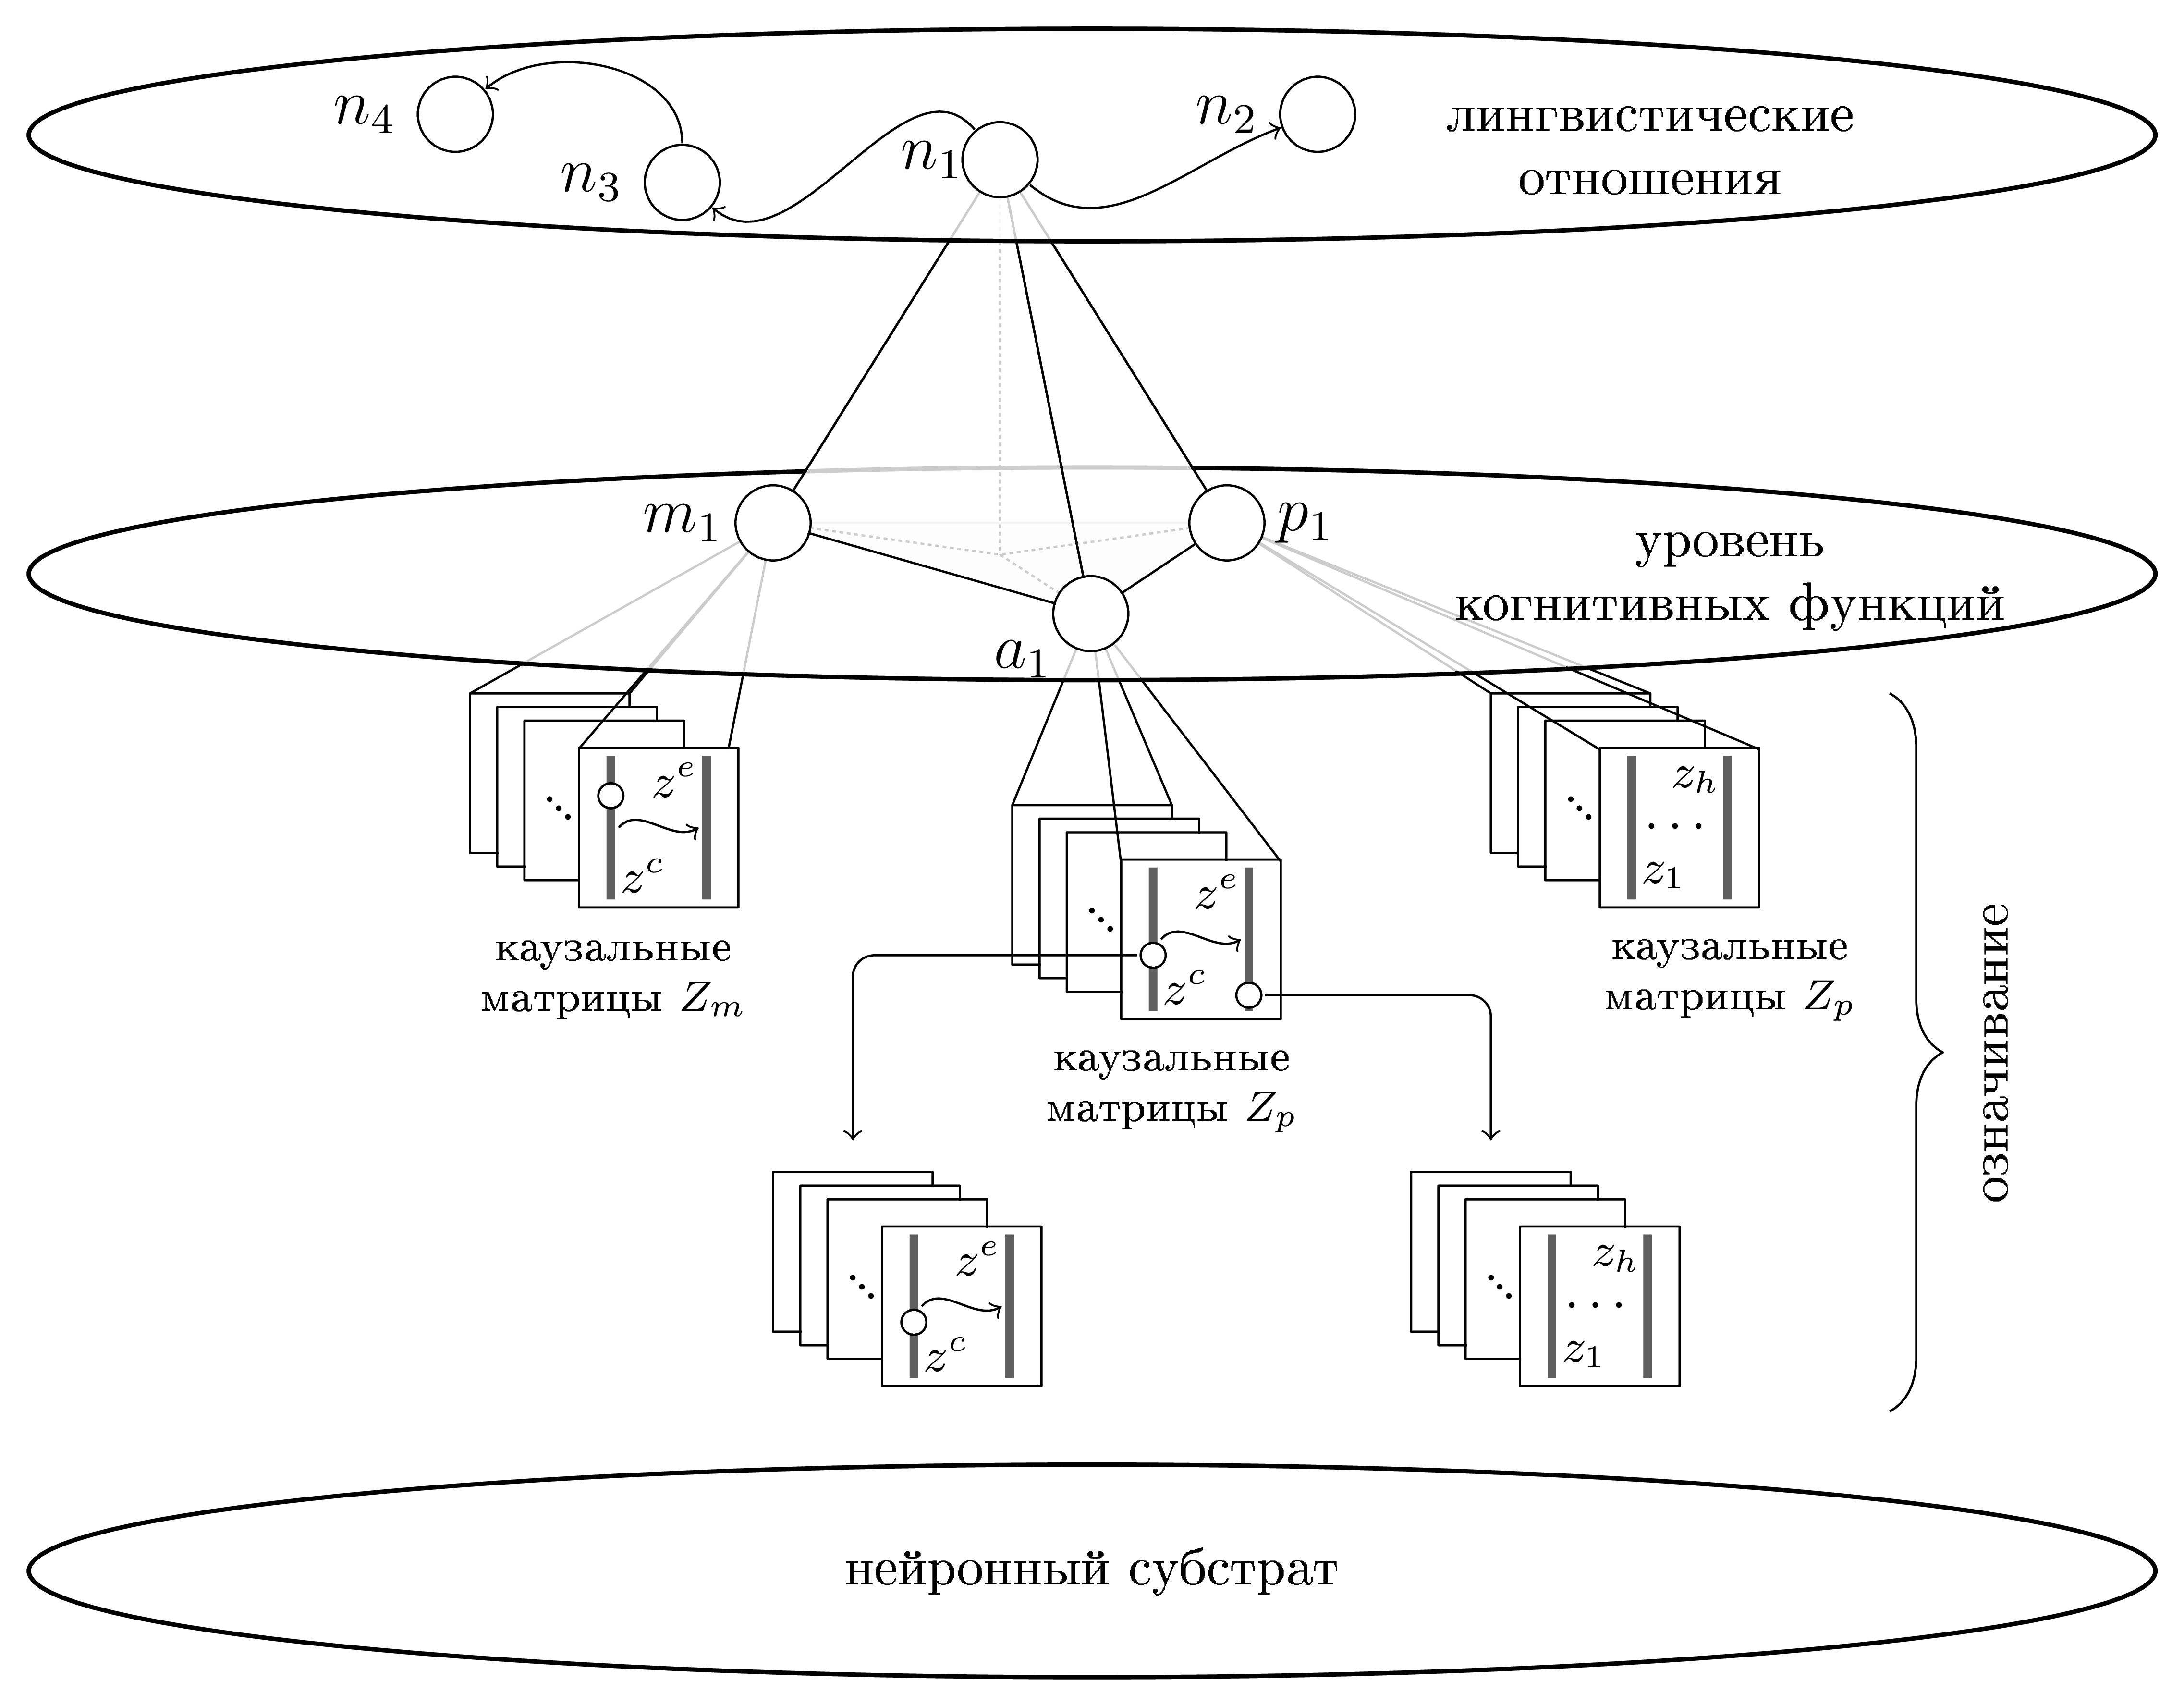
\includegraphics[width=0.7\textwidth]{signs/sign_levels}
		\end{figure}
	\end{frame}
	
	\begin{frame}
		\frametitle{Картина мира субъекта деятельности}
		
		\begin{columns}
			\begin{column}{0.55\textwidth}
				\begin{figure}
					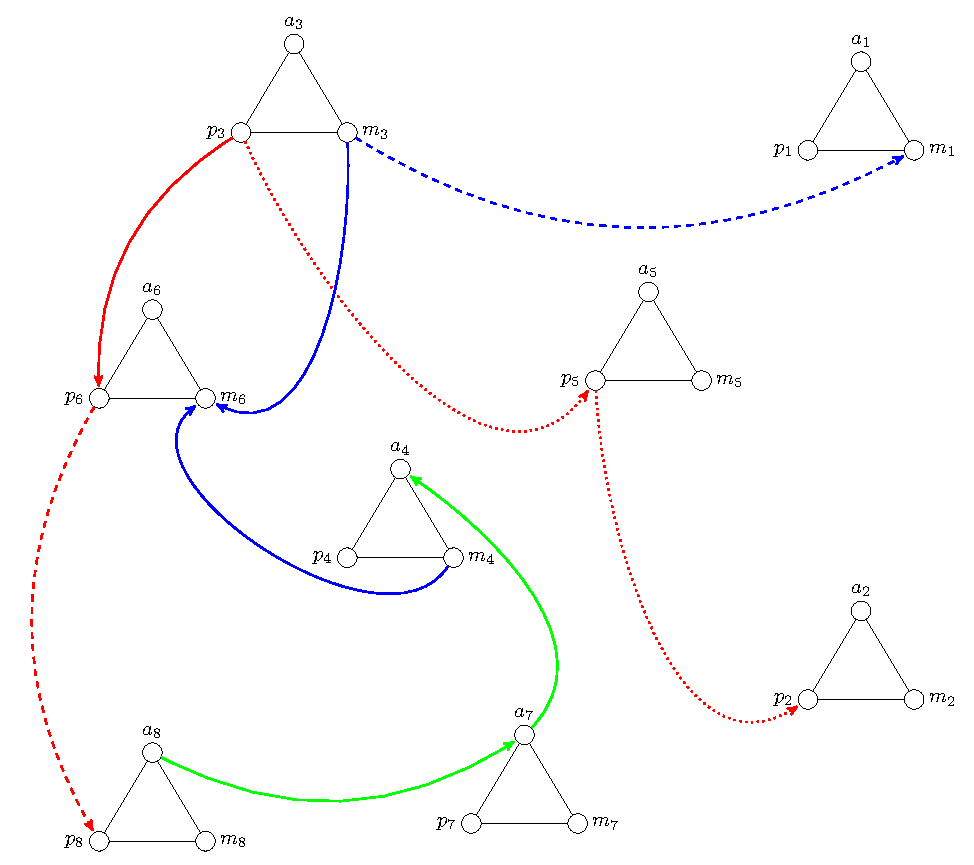
\includegraphics[width=\textwidth]{signs/signs_net}
				\end{figure}
			\end{column}
			\begin{column}{0.45\textwidth}
				\textit{Семиотическая сеть} $H=\langle H_P, H_A, H_M\rangle$, где
				\begin{itemize}
					\item $H_P=\langle2^P,\mathfrak R_P\rangle$ "--- семантическая сеть на множестве образов знаков,
					\item $H_P=\langle2^A,\mathfrak R_A\rangle$ "--- семантическая сеть на множестве значений знаков,
					\item $H_P=\langle2^M,\mathfrak R_M\rangle$ "--- семантическая сеть на множестве личностных смыслов знаков.
				\end{itemize}
			\end{column}
		\end{columns}
		\nocite{*}
		\printbibliography[keyword={signa}, resetnumbers=true]
	\end{frame}	

	\begin{frame}
		\frametitle{Образование нового знака}
		\centering
		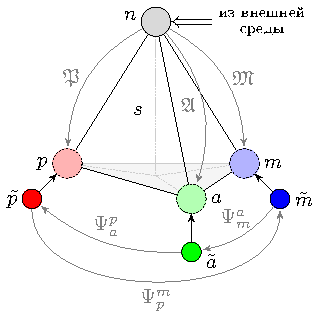
\includegraphics[width=0.5\textwidth]{signs/sign_naming_colored}
	\end{frame}		
	
	\begin{frame}
		\frametitle{Отношения на множестве компонент знака}
		\centering
		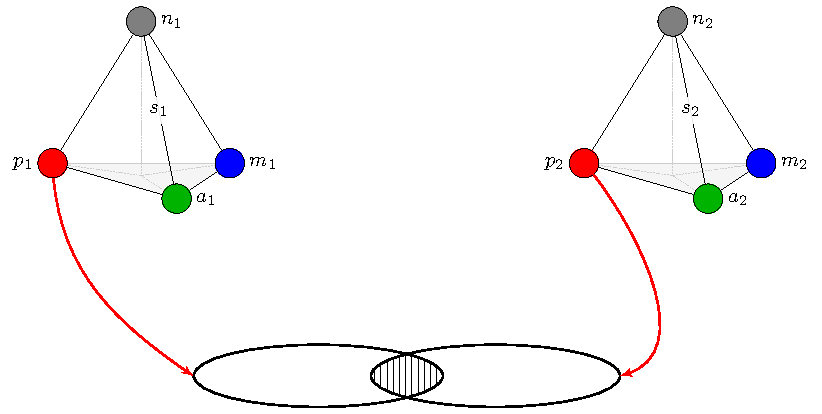
\includegraphics[page=1,width=0.8\textwidth]{signs/sign_relations}
		
		Сходство образов
	\end{frame}	
	
	\begin{frame}
		\frametitle{Отношения на множестве компонент знака}
		
		\begin{columns}
			\begin{column}{0.3\textwidth}
				\centering
				Включение образов 
				\par\bigskip
				\par\bigskip
				\par\bigskip
				\par\bigskip
				\par\bigskip
				Противопоставление образов 
				
			\end{column}
			\begin{column}{0.7\textwidth}
				\includegraphics[page=2,width=0.8\textwidth]{signs/sign_relations}
				
				\includegraphics[page=3,width=0.8\textwidth]{signs/sign_relations}
			\end{column}
		\end{columns}
		
	\end{frame}	
	
	\begin{frame}
		\frametitle{Отношения на множестве компонент знака}
		\centering
		\includegraphics[page=4,width=0.7\textwidth]{signs/sign_relations}
		
		Сценарий на значениях
	\end{frame}	
	
	\begin{frame}
		\frametitle{Отношения на множестве компонент знака}
		
		\begin{columns}
			\begin{column}{0.3\textwidth}
				\centering
				Поглощение личностных смыслов 
				\par\bigskip
				\par\bigskip
				\par\bigskip
				\par\bigskip
				\par\bigskip
				Противопоставление личностных смыслов 
				
			\end{column}
			\begin{column}{0.7\textwidth}
				\includegraphics[page=5,width=0.8\textwidth]{signs/sign_relations}
				\par\bigskip
				\includegraphics[page=6,width=0.8\textwidth]{signs/sign_relations}
			\end{column}
		\end{columns}
		
	\end{frame}	
	
	\begin{frame}
		\frametitle{Операции на множестве компонент знака}
		
		\begin{columns}
			\begin{column}{0.5\textwidth}
				\centering
				\includegraphics[page=7,width=\textwidth]{signs/sign_relations}
				\par\bigskip
				Замыкание по значениям
			\end{column}
			\begin{column}{0.5\textwidth}
				\centering
				\includegraphics[page=8,width=\textwidth]{signs/sign_relations}
				\par\bigskip
				Агглютинация личностных смыслов
			\end{column}
		\end{columns}
	\end{frame}	
		
	\begin{frame}
		\frametitle{Модель функции планирование поведения}
		\centering
		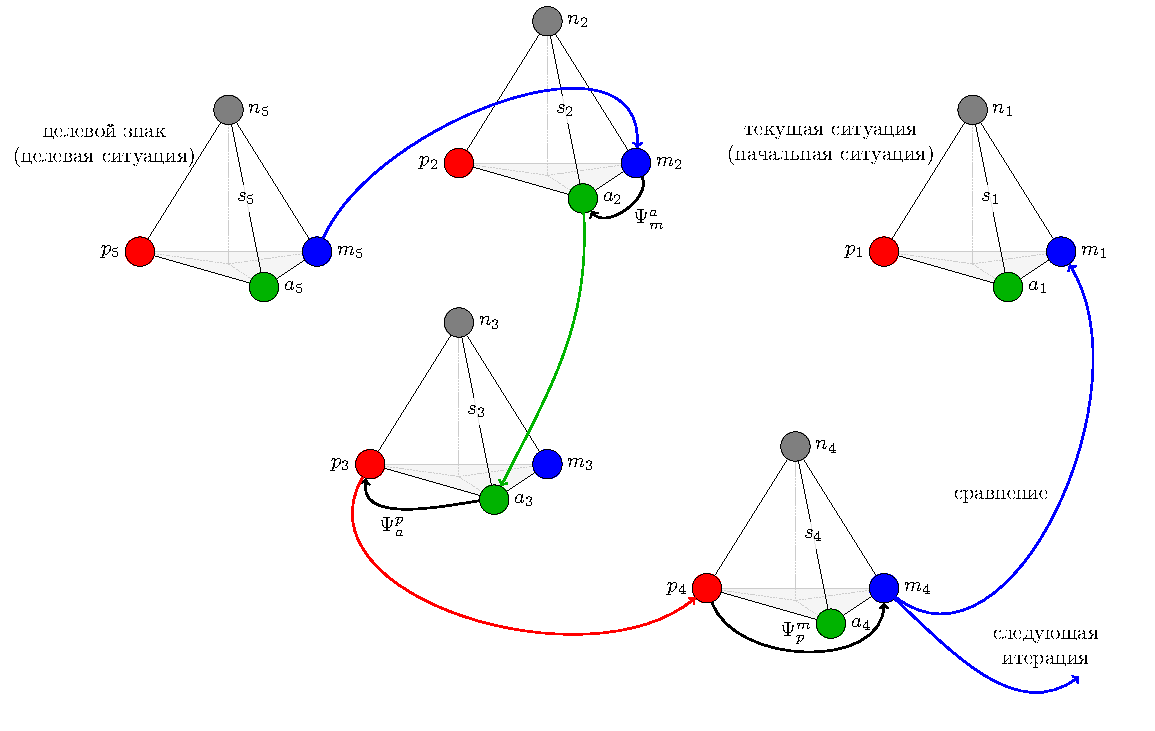
\includegraphics[width=0.9\textwidth]{algo/ru/plan_alg_ru}
		\nocite{*}
		\printbibliography[keyword={signb}, resetnumbers=true]
	\end{frame}	
	
	\section{Компоненты знака}
	\begin{frame}
		\frametitle{Модель компонент знака}
		
		\begin{columns}
			\begin{column}{0.3\textwidth}
				\begin{figure}
					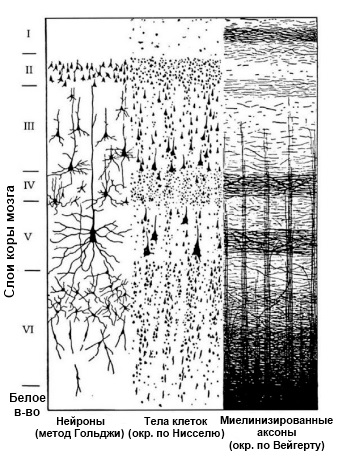
\includegraphics[width=0.5\textwidth]{phisio/column_layers_ru}
					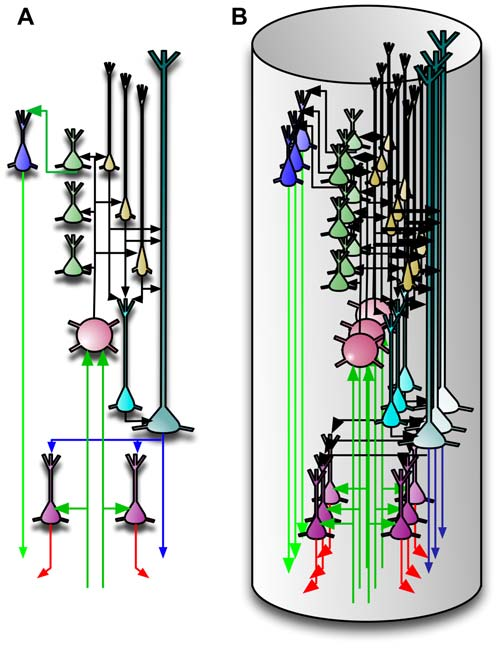
\includegraphics[width=0.5\textwidth]{phisio/column}
					\par\bigskip
					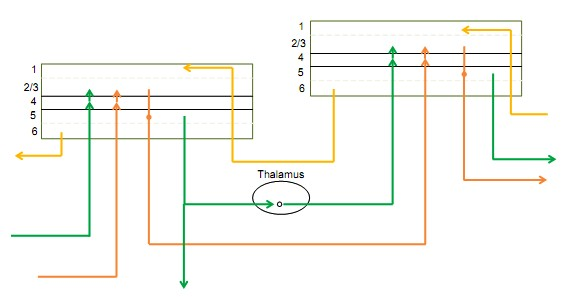
\includegraphics[width=\textwidth]{mpf/regions_connect}
				\end{figure}
			\end{column}
			\begin{column}{0.7\textwidth}
				\begin{overlayarea}{\textwidth}{0.7\textheight}
					\only<1>{
						Принимается следующие гипотезы:
						\begin{itemize}
							\item неокортекс состоит из зон (регионов), состоящих в свою очередь из колонок и имеющих одинаковое строение на всех участках коры;
							\item колонки в регионе объединены латеральными связями;
							\item таламус формирует последовательности паттернов за счет задержки возбуждения/торможения.
						\end{itemize}
					}
					
					\only<2>{
						Основные свойства:
						\begin{itemize}
							\item хранение последовательности паттернов в инвариантной форме,
							\item воспроизведение паттернов автоассоциативно,
							\item хранение паттернов в иерархической системе,
							\item использование обратной связи для предсказания поступающей на данный уровень иерархии информации. 
						\end{itemize}
					}
					
					\only<3>{
						Упрощения:
						\begin{itemize}
							\item дискретность во времени,
							\item простейшая строгая иерархия со связями только между
							ближайшими уровнями,
							\item гипотеза одинаковой длительности распознаваемых явлений в рамках одного региона,
							\item пороговая модель принятия решений в случае неопределенности результата распознавания,
							\item подавление непредвиденного сигнала,
							\item отсутствие моторной составляющей обратной связи.
						\end{itemize}
					}				
				\end{overlayarea}
			\end{column}
		\end{columns}
	\end{frame}


	\begin{frame}
		\frametitle{Модель процесса обучения}
		
		К основным принципам работы механизма обучения относятся: 
		
		\begin{itemize}
			\item использование иерархии вычислительных узлов с восходящими и нисходящими связями, 
			\item использование Хэббовских правил обучения, 
			\item разделение пространственного и временного группировщиков, 
			\item подавление второстепенной активации для формирования разреженного представления.
		\end{itemize}
		
		В результате работы механизма обучения по прецедентам (без учителя) формируются так называемые \textbf{каузальные матрицы}.
		\vfill
		\nocite{*}
		\printbibliography[keyword={htm}, resetnumbers=true]
	\end{frame}
	
	\begin{frame}
		\frametitle{Каузальная матрица}                             
		\centering
		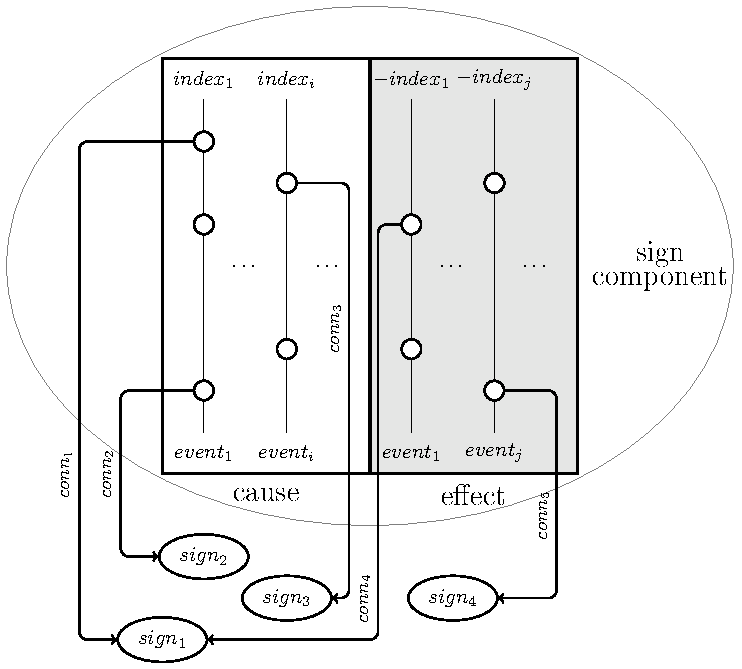
\includegraphics[width=0.4\textwidth]{automata/caus_matr}
		\vspace{10pt}
		\nocite{*}
		\printbibliography[keyword={per}, resetnumbers=true]
	\end{frame}
		
	\begin{frame}
		\frametitle{Модель процесса восприятия --- алгоритм $\mathfrak A_{th}$}
		
		\begin{tikzpicture}[overlay,remember picture]
		
		\tikzstyle{z_matrix} = [draw, rectangle, minimum width = 60, minimum height = 60,fill=white];
		
		\onslide<1->{
			\node (meas_fun) at (0.7,0.5) {$\hat f_1,\hat f_2\dots,\hat f_k$};	
		}
		\onslide<2->{
			\node (control_vect) at ($(meas_fun)+(-0.5,1.2)$) {$\hat x^{j+1}$};
			\path[->,thick,red] (control_vect.east)  edge[out = -45, in = 45, right] (meas_fun.north); 
		}
		\onslide<3->{
			\node[z_matrix] (z_1) at ($(meas_fun)+(2.6,-0.5)$) {};
			\node[z_matrix] at ($(z_1)+(0.2,-0.1)$) {};
			\node[z_matrix] at ($(z_1)+(0.4,-0.2)$) {};
			
			\node[z_matrix] at ($(z_1)+(0.9,-0.5)$) {};
			\node[z_matrix] at ($(z_1)+(1.1,-0.6)$) {};
			\node[z_matrix] at ($(z_1)+(1.3,-0.7)$) {};
			
			\path[->,thick,blue] ([xshift=20]meas_fun.south)  edge[out = -90, in = -155, right] ($(z_1)+(-1,-1.2)$);
			\path[->,thick,blue] ([xshift=-25]meas_fun.south)  edge[out = -90, in = -155, right] ($(z_1)+(-0.1,-1.7)$);
			
			\node at ($(z_1)+(-1,1.4)$) {$Z^*$};
			
			\node at ($(z_1)+(0.8,1.4)$) {$Z_1$};
			\node at ($(z_1)+(1.4,1.2)$) {$\ddots$};
			\node at ($(z_1)+(2,0.9)$) {$Z_k$};
		}
		
		\onslide<4->{
			\draw[ultra thick, green!60!black] ($(z_1)+(-0.4,-1.1)$) -- ($(z_1)+(-0.4,0.6)$);
			\draw[ultra thick, green!60!black] ($(z_1)+(0.5,-1.6)$) -- node[right,black] {$z_1^r$} ($(z_1)+(0.5,0.1)$);
			
			\draw[->, thick, green!60!black] ($(z_1)+(-0.1,-3)$) -- node[right,black] {$\bar x(0)$} ($(z_1)+(-0.1,-2)$);
		}
		
		\onslide<5->{
			\node[z_matrix] (z_2) at ($(z_1)+(5,0)$) {};
			\node[z_matrix] at ($(z_2)+(0.2,-0.1)$) {};
			
			\node[z_matrix] at ($(z_2)+(0.9,-0.5)$) {};
			\node[z_matrix] at ($(z_2)+(1.3,-0.7)$) {};
			
			\node at ($(z_2)+(-1,1.4)$) {$Z^*$};
			\node at ($(z_2)+(0.8,1.4)$) {$Z_1$};
			\node at ($(z_2)+(1.4,1.2)$) {$\ddots$};
			\node at ($(z_2)+(2,0.9)$) {$Z_k$};
			
			\draw[->, ultra thick] ($(z_1)+(2.6,-0.6)$) -- node [above] {\scriptsize$\frac{\|\bar z_1^r-\bar x(0)\|}{\|\bar z_1^r\|+\|\bar x(0)\|}$} ($(z_1)+(3.7,-0.6)$);
			
			\draw[ultra thick, dotted, green!60!black] ($(z_2)+(-0.6,-1)$) -- ($(z_2)+(-0.6,0.7)$);
			\draw[ultra thick, dotted, green!60!black] ($(z_2)+(0.5,-1.6)$) -- ($(z_2)+(0.5,0.1)$);
		}
		
		
		\onslide<6->{
			\draw[->, thick, red] ($(z_2)+(0.3,1.4)$) -- node[right,black] {$\bar x^*(0)$} ($(z_2)+(0.3,3)$);
		}
		
		\onslide<7>{
			\draw[<-, thick, red] ($(z_2)+(-0.1,-3)$) -- node[right,black] {$\hat x^j(0)$} ($(z_2)+(-0.1,-2)$);
		}
		
		\onslide<7->{				
			\draw[ultra thick, green!60!black] ($(z_2)+(-0.4,-1)$) -- ($(z_2)+(-0.4,0.7)$);
			\draw[ultra thick, green!60!black] ($(z_2)+(0.7,-1.6)$) -- node[right,black] {$z_2^r$} ($(z_2)+(0.7,0.1)$);	
		}
		\onslide<8->{
			\draw[->, thick, green!60!black] ($(z_2)+(-0.1,-3)$) -- node[right,black] {$\bar x(1)$} ($(z_2)+(-0.1,-2)$);
		}
		
		\onslide<9->{
			\draw[->, ultra thick] ($(z_2)+(2.6,-0.6)$) -- node [above] {\scriptsize$\frac{\|\bar z_1^r-\bar x(1)\|}{\|\bar z_1^r\|+\|\bar x(1)\|}$} ($(z_2)+(3.7,-0.6)$);
		}
		\end{tikzpicture}

	\end{frame}

	\section{Алгоритм планирования поведения}
	\begin{frame}
		\frametitle{Алгоритм планирования поведения}
		
		\begin{columns}
			\begin{column}{0.6\textwidth}
				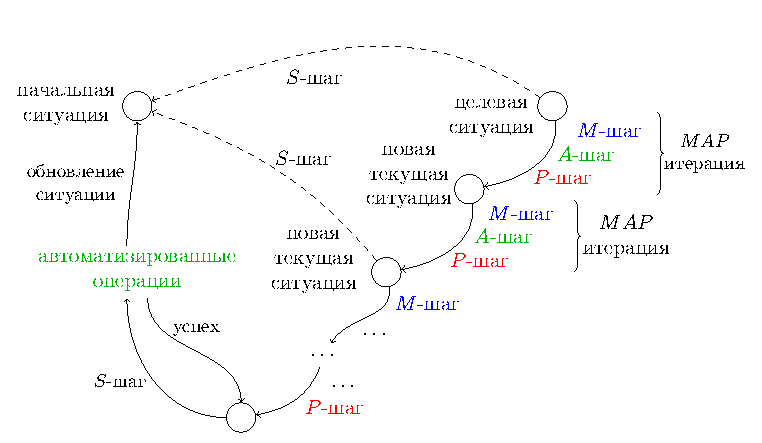
\includegraphics[width=\textwidth]{algo/ru/beh_plan2_ru}
				\vspace{20pt}
				\nocite{*}
				\printbibliography[keyword={plan}, resetnumbers=true]
			\end{column}
			\begin{column}{0.4\textwidth}
				\scriptsize
				Иерархический процесс планирования начинается с конченой ситуации и стремится достичь начальной ситуации.
				\par\bigskip
				MAP-итерация:
				\begin{itemize}
					\item \textit{M-step} -- поиск применимых действий на сети значений,
					\item \textit{A-step} -- генерация личностных смыслов, соответствующих найденным значениям,
					\item \textit{P-step} -- построение новой текущей ситуации по множеству признаков условий найденных действий,
					\item \textit{S-step} -- отправка сообщения другим участникам коалиции или выполнение найденного действия или активаций иерархии операция вплоть до автоматических операций.
				\end{itemize}
			\end{column}
		\end{columns}
		
	\end{frame}	

	\begin{frame}
		\frametitle{Пример: фрагмент сети на значениях}
		\begin{columns}
			\begin{column}{0.7\textwidth}
				\centering
				\includegraphics[page=2,width=\textwidth]{plan/plan_nets}
			\end{column}
			\begin{column}{0.3\textwidth}
				\centering
				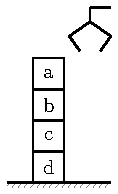
\includegraphics[page=1,width=\textwidth]{plan/block_world}
			\end{column}
		\end{columns}
	\end{frame}	

	\begin{frame}
		\frametitle{Пример: сеть на личностных смыслах - начальная ситуация}
		\begin{columns}
			\begin{column}{0.7\textwidth}
				\centering
				\includegraphics[page=3,width=\textwidth]{plan/plan_nets}
			\end{column}
			\begin{column}{0.3\textwidth}
				\centering
				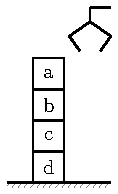
\includegraphics[page=1,width=\textwidth]{plan/block_world}
			\end{column}
		\end{columns}
	\end{frame}	

	\begin{frame}
		\frametitle{Пример: сеть на личностных смыслах - целевая ситуация}
		\centering
		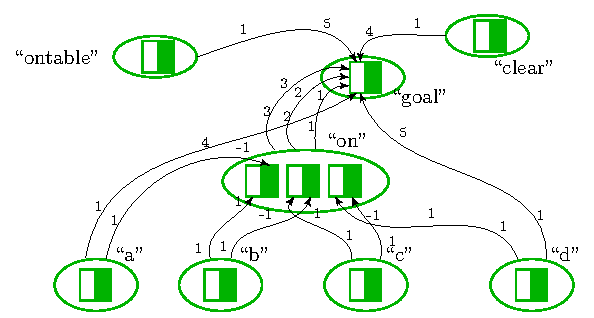
\includegraphics[page=1,width=0.7\textwidth]{plan/plan_nets}
		\par\bigskip
		\includegraphics[page=2,width=0.5\textwidth]{plan/block_world}
	\end{frame}	

	\begin{frame}
		\frametitle{Пример: фрагмент сети на значениях}
		\begin{columns}
			\begin{column}{0.7\textwidth}
				\centering
				\includegraphics[page=5,width=\textwidth]{plan/plan_nets}
			\end{column}
			\begin{column}{0.3\textwidth}
				\centering
				\includegraphics[page=3,width=\textwidth]{plan/block_world}
			\end{column}
		\end{columns}
	\end{frame}
	
	\begin{frame}
		\frametitle{Пример: генерация личностного смысла}
		
		\begin{tikzpicture}[overlay,remember picture,xshift=165pt,yshift=-50pt]
			\onslide<1->{
				\tikzstyle{ell}=[draw, thick, align=center, color=blue]
				\tikzstyle{ellf}=[draw, thick, align=center, color=blue, fill=blue]
				
				\node[ell, ellipse, minimum height = 30, minimum width = 100] (block) at (5 pt,0){};
				\predmatr{-30}{0}{block1}
				\predmatr{-10}{0}{block2}
				\predmatr{10}{0}{block3}	
				\predmatr{30}{0}{block4}
				\node at (35 pt, 20 pt) {<<block>>};
				
				\node[ell, ellipse, minimum height = 20, minimum width = 40] (c) at (32.5 pt, -50 pt){};
				\predmatr{30}{-50}{c1}
				\node at (10 pt, -35 pt) {<<c>>};		
				
				\node[ell, ellipse, minimum height = 20, minimum width = 40] (d) at (82.5 pt, -50 pt){};
				\predmatr{80}{-50}{d1}			
				\node at (60 pt, -35 pt) {<<d>>};	
				
				\node[ell, ellipse, minimum height = 20, minimum width = 40] (x) at (-37.5 pt, 50 pt){};
				\predmatr{-40}{50}{x1}
				\node at (-85 pt, 50 pt) {<<block?x>>};			
				
				\node[ell, ellipse, minimum height = 20, minimum width = 40] (y) at (42.5 pt, 50 pt){};
				\predmatr{40}{50}{y1}	
				\node at (85 pt, 50 pt) {<<block?y>>};
				
				\path[-latex'] (c.north) edge [out = 90, in = -80] node[above, black] {\scriptsize 1} node[above, black, near start] {\scriptsize 1} ([xshift=-3]block3.south);
				\path[-latex'] (d.north) edge [out = 90, in = -80] node[above, black, near end] {\scriptsize 1} node[above, black, near start] {\scriptsize 1} ([xshift=-3]block4.south);	
			}
			\onslide<1>{
				\node[ell, ellipse, minimum height = 20, minimum width = 40] (a) at (-77.5 pt, -50 pt){};
				\predmatr{-80}{-50}{a1}
				\node at (-100 pt, -35 pt) {<<a>>};
				
				\node[ell, ellipse, minimum height = 20, minimum width = 40] (b) at (-27.5 pt, -50 pt){};
				\predmatr{-30}{-50}{b1}
				\node at (-50 pt, -35 pt) {<<b>>};		
			}
			\onslide<1-2>{
				\path[-latex'] (a.north) edge [out = 90, in = -120] node[above, black, near end] {\scriptsize 1} node[above, black, near start] {\scriptsize 1} ([xshift=-3]block1.south);
				\path[-latex'] (b.north) edge [out = 90, in = -120] node[above, black, near end] {\scriptsize 1} node[above, black, near start] {\scriptsize 1} ([xshift=-3]block2.south);
			}			
			\onslide<1-3>{
				\path[-latex'] ([xshift=-10]block.north) edge [out = 90, in = -80] node[above, black] {\scriptsize 1} node[above, black, near start] {\scriptsize 0} ([xshift=-3]x1.south);
				\path[-latex'] ([xshift=10]block.north) edge [out = 90, in = -100] node[above, black] {\scriptsize 1} node[above, black, near start] {\scriptsize 0} ([xshift=-3]y1.south);
			}
			\onslide<1-4>{
				\node[ell, ellipse, minimum height = 20, minimum width = 40] (unstack) at (2.5 pt, 100 pt){};
				\predmatr{0}{100}{unstack1}
				\node at (-15 pt, 120 pt) {<<unstack>>};
				
				\node[ell, ellipse, minimum height = 20, minimum width = 40] (on) at (-77.5 pt, 100 pt){};
				\predmatr{-80}{100}{on1}
				\node at (-115 pt, 100 pt) {<<on>>};
				
				\path[-latex'] (x.north) edge [out = 90, in = -100] node[above, black, near end] {\scriptsize -1} node[above, black, near start] {\scriptsize 1} ([xshift=2]unstack1.south);
				\path[-latex'] (y.north) edge [out = 90, in = -80] node[above, black, near end] {\scriptsize -2} node[above, black, near start] {\scriptsize 1} ([xshift=5]unstack1.south);
				\path[-latex'] (on.east) edge [out = 0, in = 180] node[above, black, near end] {\scriptsize 1} node[above, black, near start] {\scriptsize 1} ([yshift=-3]unstack1.west);
				
				\path[-latex'] ([xshift=-10]x.north) edge [out = 100, in = -140] node[above, black] {\scriptsize 1} node[above, black, very near start] {\scriptsize 1} ([xshift=-3]on1.south);	
				\path[-latex'] ([xshift=-10]y.north) edge [out = 150, in = -30] node[above, black, near end] {\scriptsize -1} node[above, black, very near start] {\scriptsize 1} ([xshift=3]on1.south);					
			}			
			\onslide<1-5>{
				\node[ell, ellipse, minimum height = 20, minimum width = 40] (holding) at (82.5 pt, 120 pt){};
				\predmatr{80}{120}{holding1}
				\node at (125 pt, 120 pt) {<<holding>>};
				
				\node[ell, ellipse, minimum height = 20, minimum width = 40] (clear) at (82.5 pt, 90 pt){};
				\predmatr{80}{90}{clear1}
				\node at (120 pt, 90 pt) {<<clear>>};
				
				\path[-latex'] (clear.west) edge [out = 180, in = 0] node[above, black, near end] {\scriptsize -2} node[above, black, near start] {\scriptsize 1} ([yshift=-3]unstack1.east);
				\path[-latex'] (holding.west) edge [out = 180, in = 0] node[above, black, near end] {\scriptsize -1} node[above, black, near start] {\scriptsize 1} ([yshift=3]unstack1.east);
				
			}
			\onslide<2->{
				\tikzstyle{ell}=[draw, thick, align=center, color=green!70!black]
				\tikzstyle{ellf}=[draw, thick, align=center, color=green!70!black, fill=green!70!black]
				
				\node[ell, ellipse, minimum height = 20, minimum width = 40] (a) at (-77.5 pt, -50 pt){};
				\predmatr{-80}{-50}{a1}
				\node at (-100 pt, -35 pt) {<<a>>};
				
				\node[ell, ellipse, minimum height = 20, minimum width = 40] (b) at (-27.5 pt, -50 pt){};
				\predmatr{-30}{-50}{b1}
				\node at (-50 pt, -35 pt) {<<b>>};
			}
			\onslide<3->{
				\path[-latex', very thick] (a.north) edge [out = 90, in = -120] node[above, black, near end] {\scriptsize 1} node[above, black, near start] {\scriptsize 1} ([xshift=-3]block1.south);
				\path[-latex', very thick] (b.north) edge [out = 90, in = -120] node[above, black, near end] {\scriptsize 1} node[above, black, near start] {\scriptsize 1} ([xshift=-3]block2.south);	
			}
			\onslide<4->{
				\path[-latex', very thick] ([xshift=-10]block.north) edge [out = 90, in = -80] node[above, black] {\scriptsize 1} node[above, black, near start] {\scriptsize 0} ([xshift=-3]x1.south);
				\path[-latex', very thick] ([xshift=10]block.north) edge [out = 90, in = -100] node[above, black] {\scriptsize 1} node[above, black, near start] {\scriptsize 0} ([xshift=-3]y1.south);
			}
			\onslide<5->{
				\node[ell, ellipse, minimum height = 20, minimum width = 40] (unstack) at (2.5 pt, 100 pt){};
				\predmatr{0}{100}{unstack1}
				\node at (-15 pt, 120 pt) {<<unstack>>};
				
				\node[ell, ellipse, minimum height = 20, minimum width = 40] (on) at (-77.5 pt, 100 pt){};
				\predmatr{-80}{100}{on1}
				\node at (-115 pt, 100 pt) {<<on>>};
				
				\path[-latex', very thick] (on.east) edge [out = 0, in = 180] node[above, black, near end] {\scriptsize 1} node[above, black, near start] {\scriptsize 1} ([yshift=-3]unstack1.west);
				
				\path[-latex', very thick] ([xshift=-10]x.north) edge [out = 100, in = -140] node[above, black] {\scriptsize 1} node[above, black, very near start] {\scriptsize 1} ([xshift=-3]on1.south);	
				\path[-latex', very thick] ([xshift=-10]y.north) edge [out = 150, in = -30] node[above, black, near end] {\scriptsize -1} node[above, black, very near start] {\scriptsize 1} ([xshift=3]on1.south);
				\path[-latex', very thick] (x.north) edge [out = 90, in = -100] node[above, black, near end] {\scriptsize -1} node[above, black, near start] {\scriptsize 1} ([xshift=2]unstack1.south);
				\path[-latex', very thick] (y.north) edge [out = 90, in = -80] node[above, black, near end] {\scriptsize -2} node[above, black, near start] {\scriptsize 1} ([xshift=5]unstack1.south);	
			}
			\onslide<6->{
				\node[ell, ellipse, minimum height = 20, minimum width = 40] (holding) at (82.5 pt, 120 pt){};
				\predmatr{80}{120}{holding1}
				\node at (125 pt, 120 pt) {<<holding>>};
				
				\node[ell, ellipse, minimum height = 20, minimum width = 40] (clear) at (82.5 pt, 90 pt){};
				\predmatr{80}{90}{clear1}
				\node at (120 pt, 90 pt) {<<clear>>};
				
				\path[-latex', very thick] (clear.west) edge [out = 180, in = 0] node[above, black, near end] {\scriptsize -2} node[above, black, near start] {\scriptsize 1} ([yshift=-3]unstack1.east);
				\path[-latex', very thick] (holding.west) edge [out = 180, in = 0] node[above, black, near end] {\scriptsize -1} node[above, black, near start] {\scriptsize 1} ([yshift=3]unstack1.east);
			}			
		\end{tikzpicture}
	\end{frame}
	
	\begin{frame}
		\frametitle{Пример: генерация личностного смысла}
		\begin{columns}
			\begin{column}{0.7\textwidth}
				\centering
				\includegraphics[page=4,width=\textwidth]{plan/plan_nets}
			\end{column}
			\begin{column}{0.3\textwidth}
				\centering
				\includegraphics[page=3,width=\textwidth]{plan/block_world}
			\end{column}
		\end{columns}
	\end{frame}
				
	\section{Задача интеллектуального перемещения}
	\begin{frame}
		\frametitle{Особенности постановки задачи}
		
		Рассматривается случай группового взаимодействия автономных технических объектов (агентов), в котором:
		\begin{itemize}
			\item агенты решают общую задачу (имеют общую цель высшего уровня),
			\item агенты действуют независимо друг от друга (децентрализованное управление), в т.ч. могут ставить индивидуальные подцели и достигать их,
			\item агенты обладают различными характеристиками, как техническими, так и когнитивными, т.е. разными стратегиями поведения,
			\item агенты обладают различными картинами мира,
			\item агенты действуют в меняющейся среде.
		\end{itemize}
		
	\end{frame}
	
	\begin{frame}
		\frametitle{Требования к представлению знаний}
		
		На представление пространственных и временных знаний в задаче согласованного перемещения с такими особенностями налагается ряд ограничений:
		\begin{itemize}
			\item необходимость поддержки некоторого протокола коммуникации, разделение знаний на коммуницируемые и некоммуницируемые (личные),
			\item необходимость выделения компоненты знания, не зависящей от индивидуальных (личных) характеристик агента,
			\item требование к наличию механизма связывания реальных объектов внешней среды и процедур их распознавания с символьным коммуницируемым представлением (symbol grounding problem),
			\item поддержка механизмов пополнения картины мира (обучение и абстрагирование).
		\end{itemize}
	\end{frame}
		
	\begin{frame}
		\frametitle{Задача интеллектуального перемещения}
		
		\begin{columns}
			\begin{column}{0.55\textwidth}
				\begin{center}
					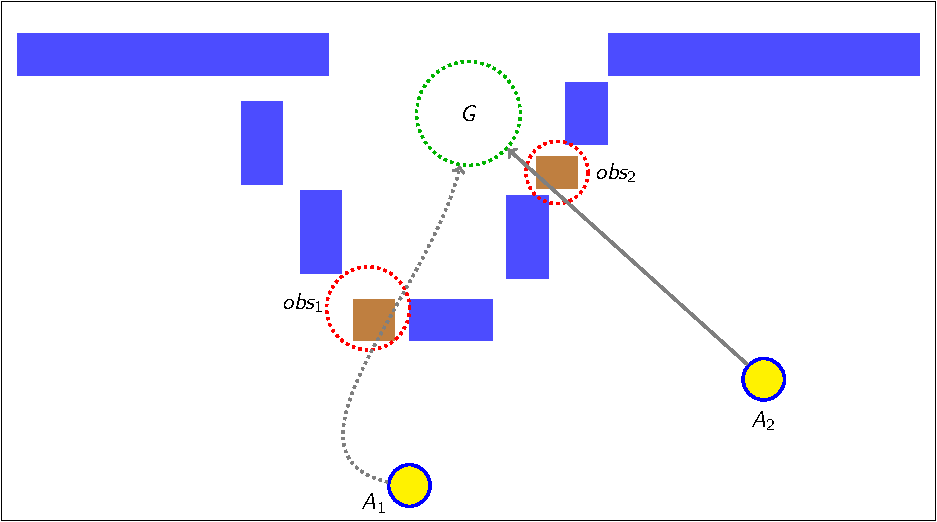
\includegraphics[page=1,width=0.8\textwidth]{examples/slides_colored}
				\end{center}
				\vspace{-7pt}
				\small
				\textbf{Задача}
				
				Целевая область не достижима некоторым агентом самостоятельно (с использованием только методов планирования траектории).
				
				\textbf{Решение}
				
				Агенты должны поддерживать коммуникацию и модифицировать свои собственные планы с учетом коалиционных подзадач.
				
			\end{column}
			\begin{column}{0.45\textwidth}
				Особенности:
				\begin{itemize}
					\item Меняющаяся внешняя среда.
					\item Различные типы препятствий (некоторые могут быть разрушены).
					\item Агенты обладают различной функциональностью.
					\item Общая пространственная цель (ВСЕ агенты должны достичь определенной области на карте).
				\end{itemize}
			\end{column}
		\end{columns}
	\end{frame}
	
	\begin{frame}
		\frametitle{Представление пространственных знаний}
		
		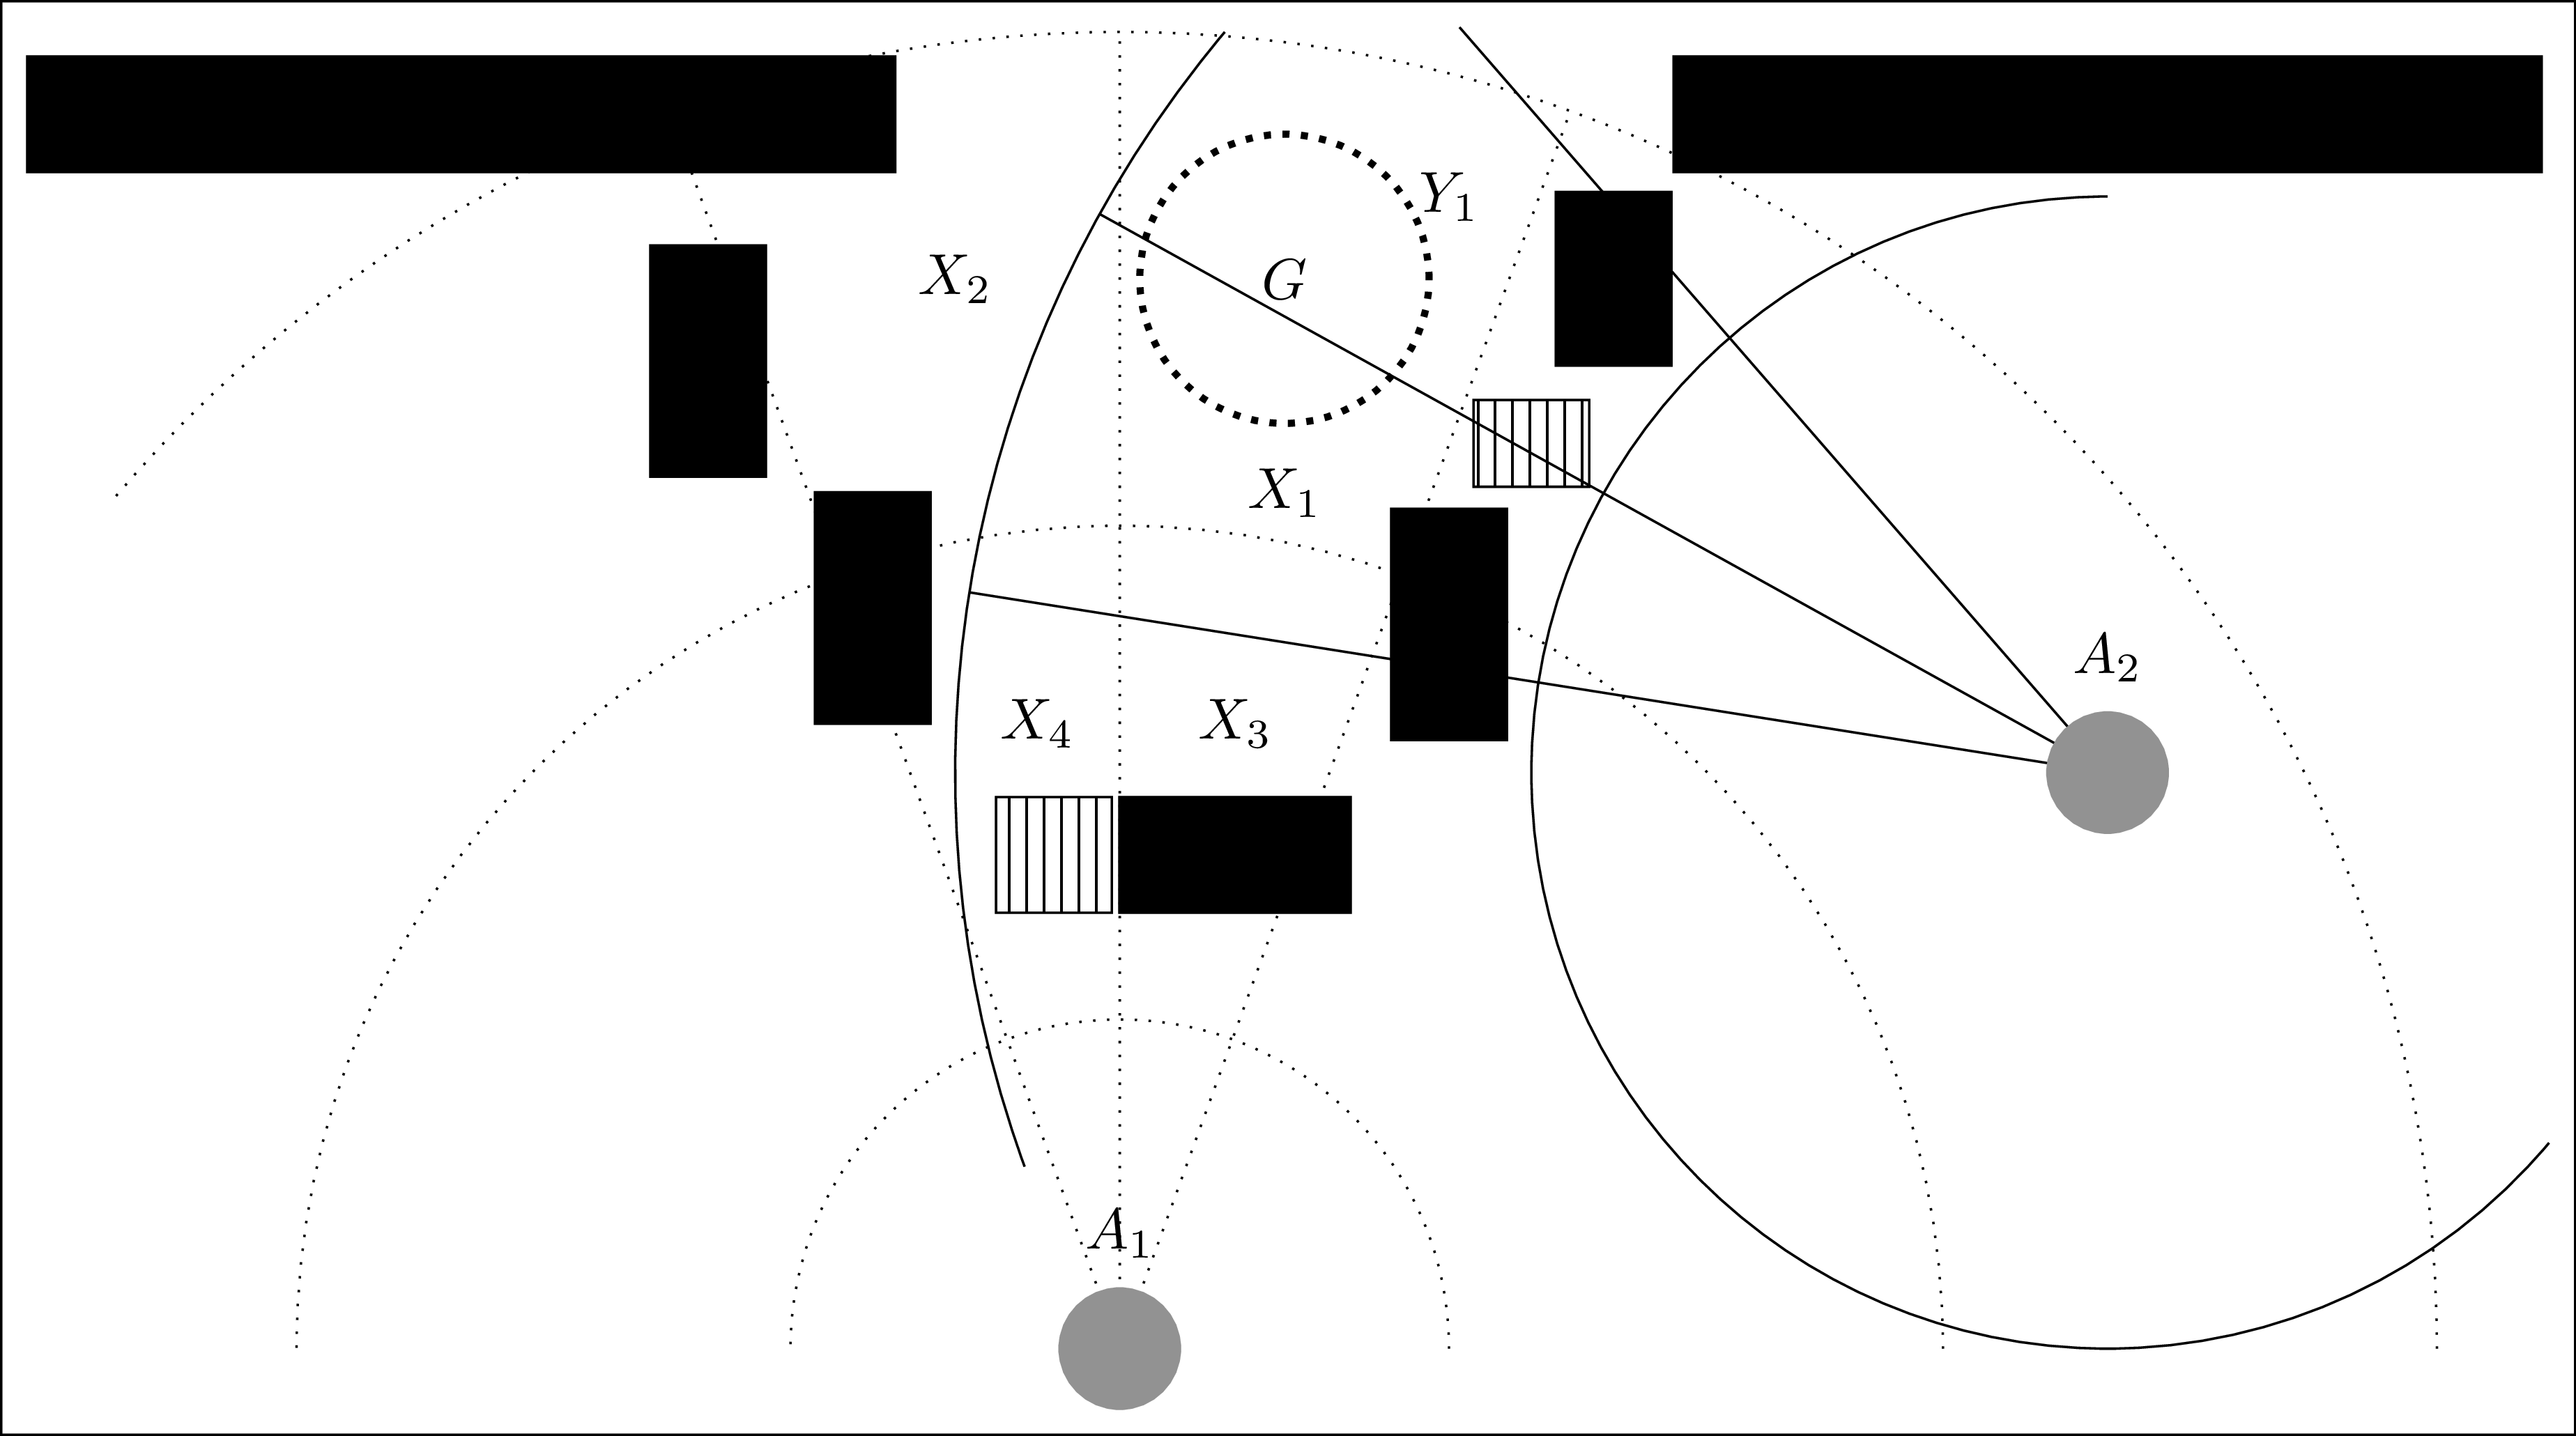
\includegraphics[width=\textwidth]{examples/rita_ex_proc.png}
		
		\nocite{*}
		\printbibliography[keyword={planknow}, resetnumbers=true]
	\end{frame}
	
	\begin{frame}
		\frametitle{Представление действий по перемещению}
		
		Действия по перемещению "--- знаки $s_t$ (признаки $f_t$, $t$ "--- тип перемещения), которым соответствуют каузальные матрицы типа $Z_t$, состоящие из трёх столбцов 
		\[
		z_1=(l_x, I), z_2=(l_y, d_u, E), z_3=(l_y, I, t_v),
		\]
		где 
		\begin{itemize}
			\item $l_x$, $l_y$ "--- признаки, соответствующие категории расстояния в пространственной логике  (например, вплотную, близко, далеко и др.), 
			\item $d_u$ "--- признак, соответствующий категории направления в пространственной логике (например, впереди, слева и др.), 
			\item $t_v$ "--- признак, соответствующий категории времени во временной логике (например, скоро, в будущем и др.),
			\item $I$ "--- признак присутствия самого агента, 
			\item $E$ "--- признак отсутствия препятствия.
		\end{itemize}
	\end{frame}	
	
	\begin{frame}
		\frametitle{Распределение ролей при решении задачи}
		\begin{center}
			\scalebox{0.7}{
				\animategraphics{12}{examples/slides_colored}{}{}			
			}
		\end{center}
	\end{frame}
	
	\begin{frame}
		\frametitle{Пример по перемещению}
		
		\begin{center}
			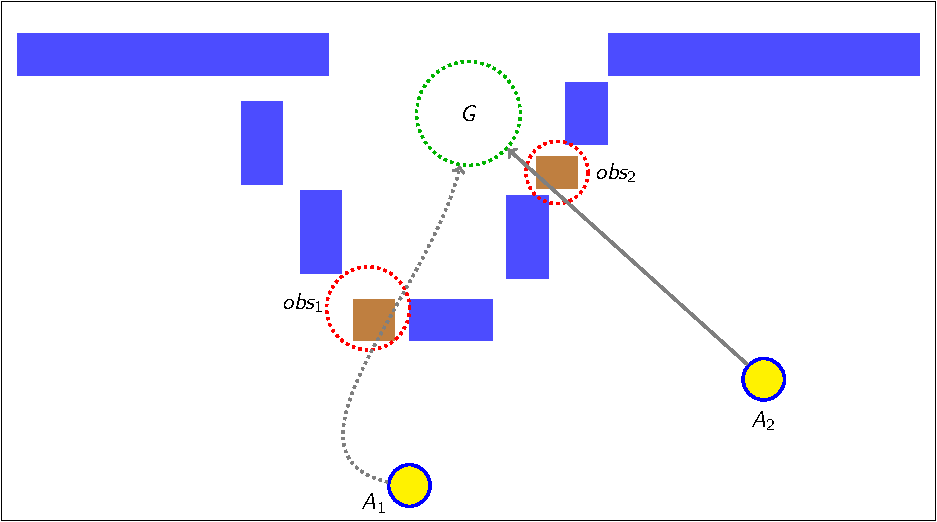
\includegraphics[page=1,width=0.85\textwidth]{examples/slides_colored}
		\end{center}
		\par\bigskip
		Актуализированные знаки агента $A_1$: ``область $X_6$'', ``далеко'', ``перемещение 1'' $\rightarrow$ \color{green!70!black} операции планирования траектории.
	\end{frame}
	
	\begin{frame}
		\frametitle{Пример по перемещению}
		
		\begin{center}
			\includegraphics[page=31,width=0.85\textwidth]{examples/slides_colored}
		\end{center}
		\par\bigskip
	Актуализированные знаки агента $A_1$: ``препятствие 1'', ``рядом'', ``область $X_6$''.
	\end{frame}
	
	\begin{frame}
		\frametitle{Пример по перемещению}
		
		\begin{center}
			\includegraphics[page=42,width=0.85\textwidth]{examples/slides_colored}
		\end{center}
		\par\bigskip
		Актуализированные знаки агента $A_1$: ``отправить сообщение'', ``агент $A_2$''.
	\end{frame}
	
	\begin{frame}
		\frametitle{Пример по перемещению}
		
		\begin{center}
			\includegraphics[page=58,width=0.85\textwidth]{examples/slides_colored}
		\end{center}
		\par\bigskip
		Актуализированные знаки агента $A_2$: ``область $Y_3$'', ``далеко'', ``перемещение 2'' $\rightarrow$ \color{green!70!black} операции планирования траектории.
	\end{frame}
	
	\begin{frame}
		\frametitle{Пример по перемещению}
		
		\begin{center}
			\includegraphics[page=95,width=0.85\textwidth]{examples/slides_colored}
		\end{center}
		\par\bigskip
		Актуализированные знаки агента $A_2$: ``область $Y_1$'', ``рядом'', ``препятствие 1'', ``разрушить''.
	\end{frame}
	
	\begin{frame}
		\frametitle{Пример по перемещению}
		
		\begin{center}
			\includegraphics[page=116,width=0.85\textwidth]{examples/slides_colored}
		\end{center}
		\par\bigskip
		Актуализированные знаки агента $A_1$ and $A_2$: ``далеко'', ``перемещение 3'' $\rightarrow$ \color{green!70!black} операции планирования траектории.
	\end{frame}
	
	\begin{frame}
		\frametitle{Пример по перемещению}
		
		\begin{center}
			\includegraphics[page=171,width=0.85\textwidth]{examples/slides_colored}
		\end{center}
		\par\bigskip
		Актуализированные знаки агента $A_1$ и $A_2$: целевое состояние (``область $G$'').
	\end{frame}
			
	\begin{frame}
		\frametitle{Применение для решения интеллектуальных задач}
		\vspace{-5pt}
		\footnotesize
		\begin{columns}
			\begin{column}{0.5\textwidth}
				\begin{itemize}
					\item Моделирование внимания.
					\item Образование нового знания (концепта).
					\item Планирование поведения.
					\item Построение картины мира субъекта на основе текстов.
					\item Генерация сообщений на основе картин мира определенного типа (виртуальные ассистенты).
					\item Построение многоуровневых архитектур управления.
				\end{itemize}
				
			\end{column}
			\begin{column}{0.3\textwidth}
				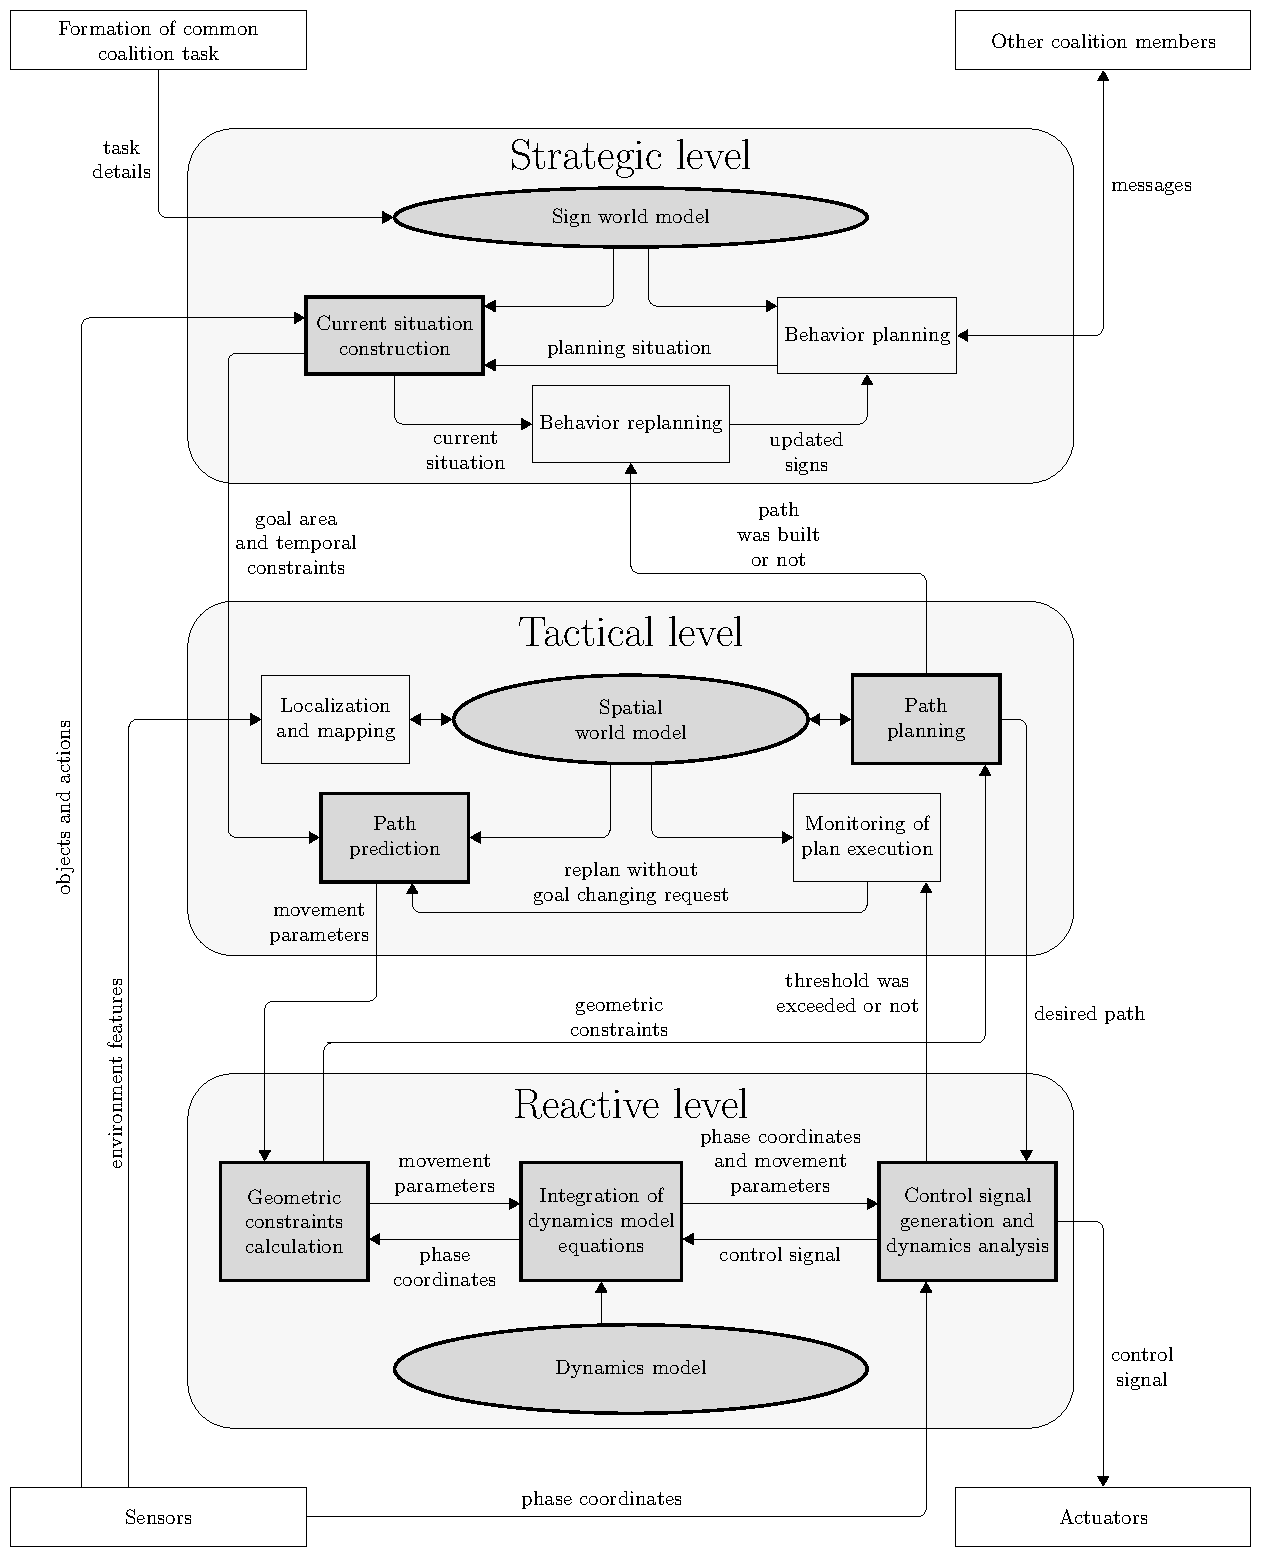
\includegraphics[width=\textwidth]{strl/strl_arch_real_eng}
			\end{column}
			\begin{column}{0.2\textwidth}
				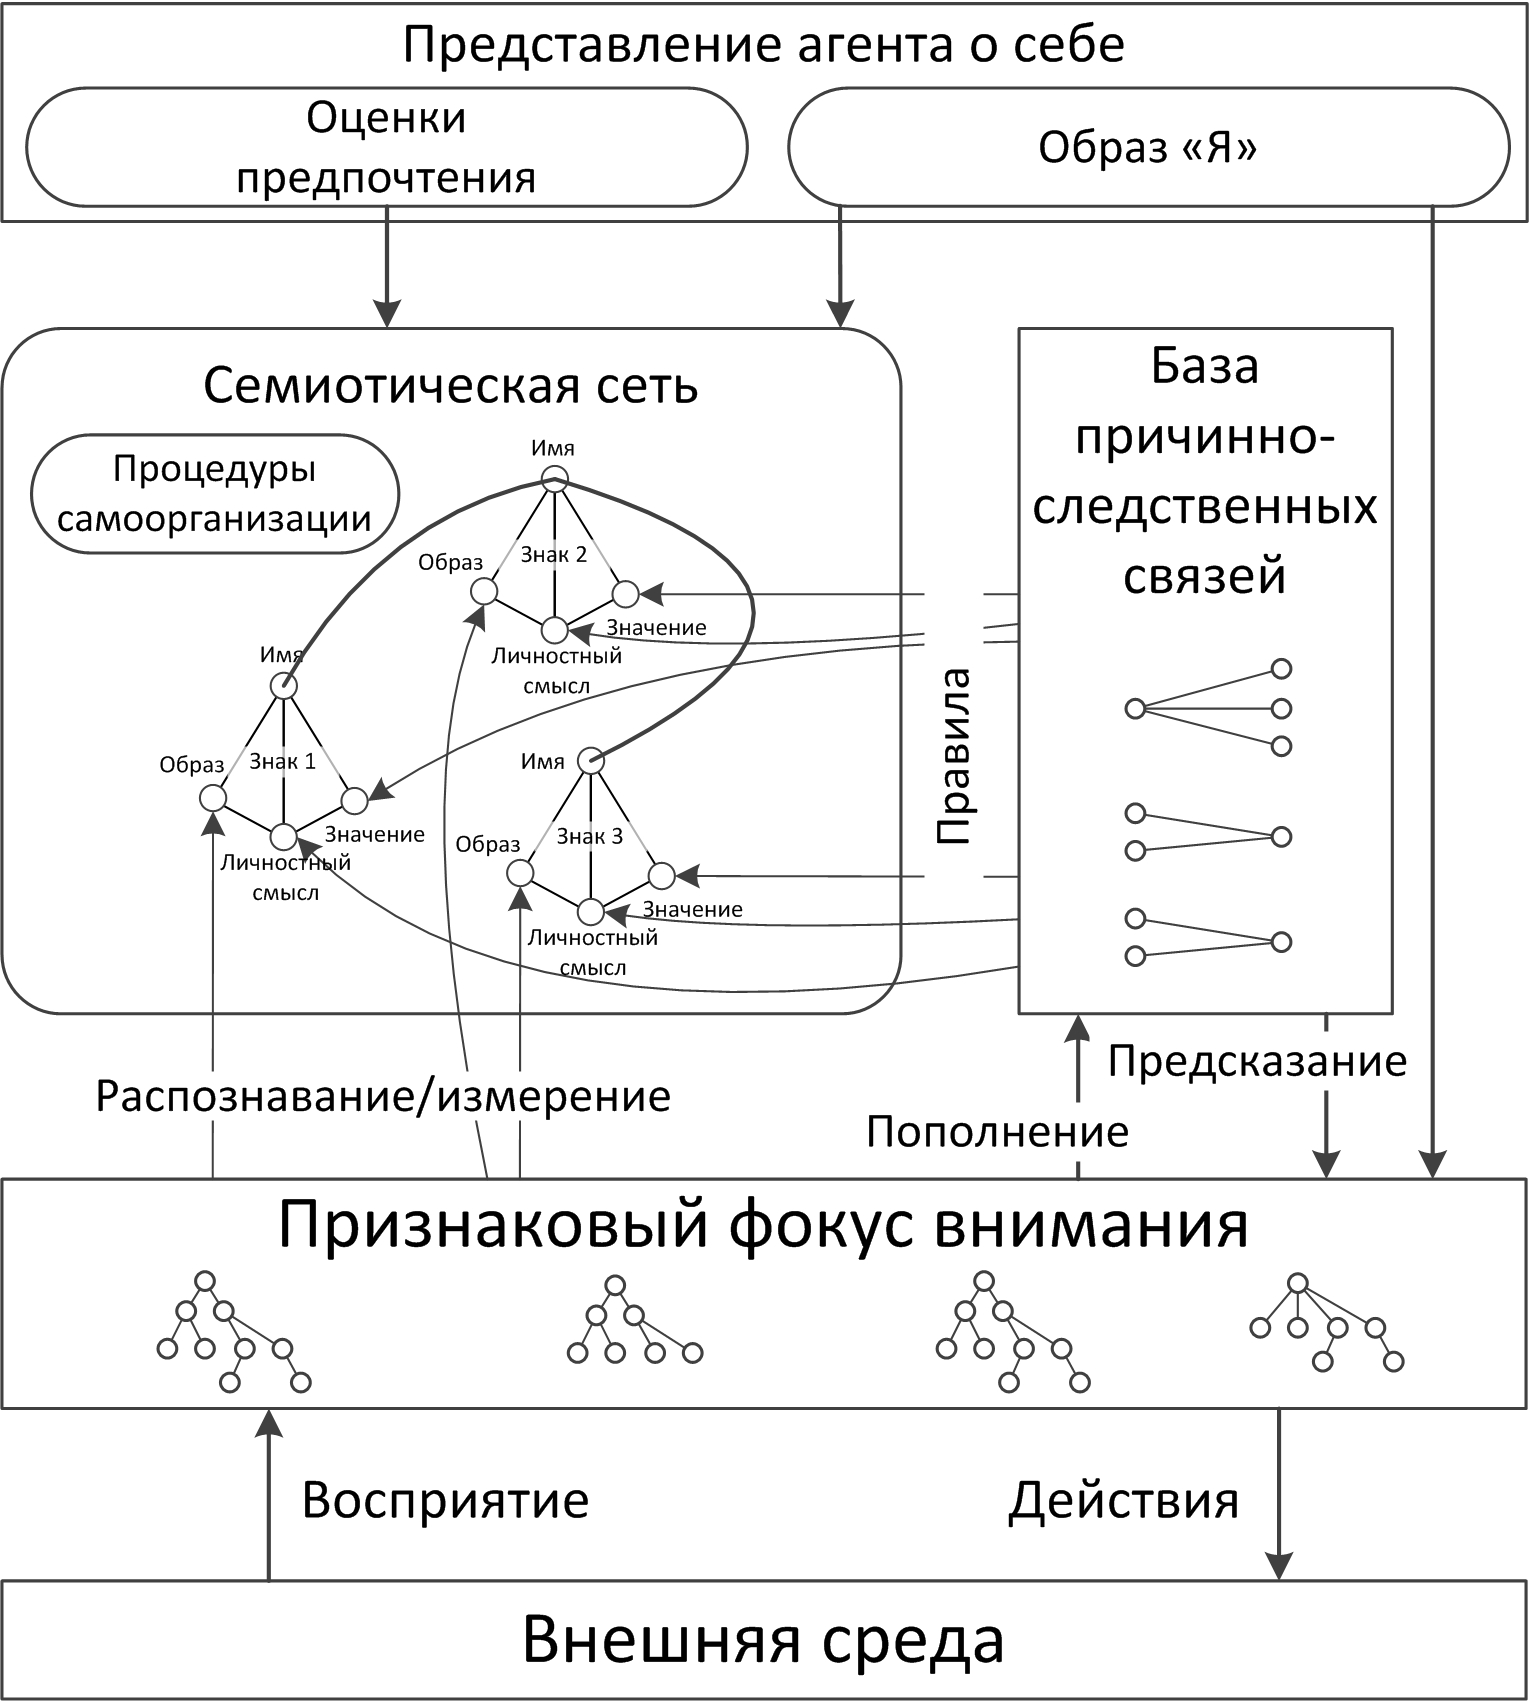
\includegraphics[width=\textwidth]{signs/iagent}
			\end{column}
			
		\end{columns}
		\vspace{-5pt}
		\nocite{*}
		\printbibliography[keyword={strl}, resetnumbers=true]
	\end{frame}

	\begin{frame}
		\centering
		\Huge
		Спасибо за внимание!
		\normalsize
		\par\bigskip
		\par\bigskip
		ФИЦ ИУ РАН, лаб. <<Динамические интеллектуальные системы>>, pan@isa.ru
		\par\bigskip
		\par\bigskip
		\url{https://github.com/cog-isa/map-planner.git}
	\end{frame}
	
\end{document}
	
	
